\section{A World Model Must Survive Its Own Actions}

A map is useful because it leaves things out. A road map omits the grain of the asphalt. A robot's contact model may omit the building's architecture. A clinician's model of an intervention cannot track every molecule in a patient's body. The question is which omissions remain harmless when someone acts on the model.

A world model earns its name through the expectations it makes available: what is likely to happen, which action may change it, what evidence should be collected next, and when the model has ceased to be adequate. It need not be a miniature universe inside a machine.

\subsection{Building the Model While Using It}

A demand for complete understanding before useful action would stop nearly every practical learner. People learn a tool while using it. A mobile robot can estimate its position while constructing a map. An agent can discover a software environment by inspecting files, running commands, and interpreting the results.

This is a bootstrapping problem. The provisional model guides an action; the action produces evidence; the evidence revises the model. The quality of the loop matters more than the completeness of the initial representation.

The difficulty of hand-building comprehensive representations was already visible in ambitious knowledge-based computing programs. Japan's Fifth Generation Computer Systems project pursued parallel inference and logic programming, producing research and working systems without establishing the broad industrial transformation its most expansive expectations anticipated \cite{aiso1988fifth,feigenbaum1993japanese}. A useful historical lesson is the cost of maintaining explicit knowledge as coverage expands. Its useful legacy is the question of how representations stay current as coverage expands.

Contemporary digital agents distribute the burden. The model supplies hypotheses and plans. A repository supplies persistent state. Logs supply memory of what occurred. Tools supply exact calculations and executable observations. A test suite supplies a partial judge. Some of what an agent “knows” lives in its ability to recover the right external state when needed.

Embodied systems face the same architecture with a heavier interface. Touch, force, position, contact history, wear, and time enter the loop. A cup does not interpret a robot's intentions. It does retain the consequences of being pushed. The next action meets the cup where the previous action left it.

Planning systems can operate above fast local controllers. A high-level model may choose a grasp or a route while lower-level loops manage forces and motion. The necessary rates depend on the hardware and task. Classic force-control research documents how sensing, mechanical dynamics, and unmodeled modes constrain useful feedback bandwidth \cite{eppinger1987}. A broad claim that “the robot runs at a kilohertz” can conceal several nested loops with different jobs.

By July 2026, Google's Gemini Robotics 2 work explicitly brought high-level embodied capabilities together with whole-body control and robot action \cite{geminirobotics2026}. The relevant advance is the connection among perception, planning, and execution. A demonstration still has a task distribution, hardware configuration, and recovery policy. Those determine what the demonstrated capability can support.

\subsection{Three Strengths of Coupling}

The cost of an inadequate model depends on how tightly its outputs are coupled to consequences.

In a loosely coupled task, a draft can be inspected before use. A translator can revise a paragraph. A developer can reject a patch. The external state need not change every time the model proposes something.

In a strong physical loop, each action changes the state encountered by the next action. A slight slip changes the grip. A delayed correction changes the contact force. Errors may persist and interact rather than reset between steps.

In a reflexive loop, other agents interpret the intervention and change strategy. A trader responds to a forecast that other traders also read. A platform's ranking rule changes the behavior of those being ranked. A policy changes the incentives under which its own evidence will be generated.

These are coupling regimes, not species of intelligence. Software can be tightly coupled to consequential infrastructure. A physical inspection can remain advisory. Social systems can have stable equilibria, unstable dynamics, or both under different conditions. Reflexivity removes the convenience of treating the observed distribution as independent of the observer's deployed policy.

One can write a simple model--action update as
\begin{equation}
 a_t=\pi(m_t),\qquad
 m_{t+1}=U(m_t,a_t)=F(m_t).
\end{equation}
Here $m_t$ denotes the current model state and $a_t$ the chosen action. The feedback derivative is the derivative of the \emph{composite} map:
\begin{equation}
 DF(m)=
 \frac{\partial U}{\partial m}
 +\frac{\partial U}{\partial a}D\pi(m).
\end{equation}
Ignoring the second term ignores the fact that changing the model changes the action used to update it.

If $F$ maps a complete invariant domain into itself and is uniformly contractive there, a fixed point exists, is unique in that domain, and iteration converges to it. A derivative smaller than one at an isolated point establishes much less; noise, delay, a changing environment, and an unmodeled state can alter the conclusion. The stability argument therefore has to cover the whole update map, its domain, and the receiving environment.

Simultaneous localization and mapping makes bootstrapping tangible. It also makes the assumptions visible: sensor geometry, observability, motion, and the treatment of moving objects affect whether a map and position estimate remain useful. A robot manipulating an object faces an additional burden because its actions deliberately change the scene. A strategic agent adds another because the scene's other occupants respond to its policy.

Across these settings, an important capability is continuity after an error. Can the system observe the new state, recover what matters, and choose another safe action? A beautiful prediction with no recovery route may be less useful than a rougher model embedded in a resilient loop.


\begin{figure}[ht]
\centering
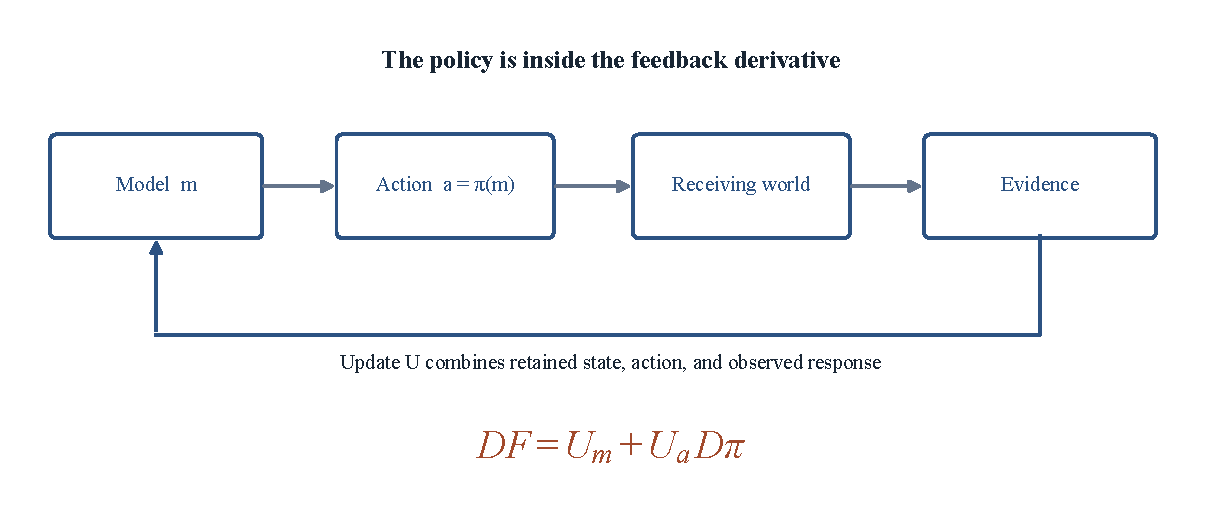
\includegraphics[width=\textwidth]{assets/model-action-loop.pdf}
\caption{The model changes the action, which changes the evidence used in the next update. $U$ combines retained state, action, and environmental response. The derivative of the composite map contains both the direct term and the path through the policy.}
\label{fig:mechanism-model-action-loop}
\end{figure}
\subsection{Compression That Supports Intervention}

Call a representation \emph{intervention-ready compression} when it preserves enough structure to guide a specified class of actions within stated error and risk tolerances. The phrase names a practical requirement. Causal inference already supplies rigorous distinctions among observation, intervention, and counterfactual reasoning \cite{pearl2009causality}.

Records can contain evidence about all three. Text is not confined to surface correlation: it can describe experiments, mechanisms, and failed interventions. A learner can recover causal structure from such records when the data and assumptions permit it. Nevertheless, accurate prediction of records alone does not certify a particular intervention model.

The transition to action asks a different question. If the system changes this variable, with these constraints and this history, how does the distribution of later states change? A drug may alter the probability of an outcome without determining every patient's response. A control signal may shift a trajectory distribution without producing identical motion on every attempt. Actionable causality does not require determinism.

Which variables must be retained? A local sensitivity screen offers one limited answer:
\begin{equation}
 \left|\frac{\partial f}{\partial x_i}\right|\sigma_i>\theta.
\end{equation}
For a scalar state-transition quantity $f$, the left side estimates the effect of uncertainty $\sigma_i$ in variable $x_i$. The threshold $\theta$ must use the same units as that effect. A variable whose estimated effect exceeds the task's tolerance deserves attention.

This is a first-order approximation. Interactions, correlated uncertainties, discontinuities, and rare severe events can defeat it. A variable can have a small local derivative and still determine whether a system crosses a catastrophic boundary. Selecting a model therefore requires more than ranking ordinary sensitivities.

Scale matters for the same reason. At one scale, friction can be represented by an effective coefficient. At another, surface texture, deformation, temperature, and contact history may have to reappear. The right representation is the one that remains useful under the interventions actually contemplated.

Simulation buys controlled variation. Real feedback tests transfer. Domain randomization, demonstrations, online learning, and model-based planning arrange this exchange differently \cite{tobin2017domain}. Their common bill includes observations of how the receiving world responds.

Those observations can be expensive and slow. In drug development, a historical estimate based on selected company data included both unsuccessful projects and the financing cost of time \cite{dimasi2016}. Such estimates are sensitive to sample and accounting choices; no single figure is the timeless price of discovering a drug. The robust point is that copying a report and obtaining a new clinical response draw on different resources.

The 2026 rentosertib program makes the distinction current. An AI-associated discovery and development process had reached a Phase III program, with the first patient announced in September \cite{insilico2026phase3}. Enrolling a trial creates a route to evidence. Its announced follow-up period is still time that has to pass. The label “AI-discovered” cannot supply the missing outcomes.

Resource barriers determine how much a real observation costs. Temporal rigidity determines when it becomes available. Topological coupling determines where an intervention's effects travel. A world model operates inside these constraints, using a limited budget of responses to improve future decisions.

Reversibility changes the budget. A discarded software hypothesis can often be recovered from a log. An unnecessary physical collision may destroy the state needed to try again. In a clinical or ecological setting, some uncertainty cannot be resolved by unrestricted experimentation. The model must then support conservative margins, staged interventions, and explicit decisions about which uncertainty remains.

Other agents complicate the target further. Once a model is deployed, people can adapt to it, exploit its categories, or withhold the evidence it expects. The representation that worked before deployment may become inadequate because deployment succeeded in changing behavior. Monitoring must therefore ask whether the transition rule itself is drifting.

Failure reveals an omission, but not every failure identifies it uniquely. A missed grasp can reflect perception, calibration, mechanics, or planning. A weak treatment response can have several explanations. Learning requires experiments and diagnostics that distinguish among them. More failed actions without better attribution can consume the feedback budget without improving the model.

The ambition is demanding and concrete: use finite, costly, noisy responses to build a representation that continues to support action after action has changed the world. A model needs to retain what the next consequential intervention will make matter.

That requirement leads directly to the body. Some of the variables a model could track are handled instead by elasticity, geometry, reflex, and metabolism. The next chapter examines this older form of compression, built into matter and paid for through evolution, development, and maintenance.
